\documentclass[tikz]{standalone}
\usetikzlibrary {automata,positioning,fit,calc} 
\usepackage{inconsolata}
 \usepackage{mathtools,amsmath}

\tikzset{%
    pics/myrec/.style n args={7}{code={%  
        \node (#1) at (0,0) [draw,#2,text=black,font=\tiny, align=center,thick,minimum width=2cm,minimum height=1cm, rounded corners,label={\tiny\{#3,#4\}}]{\textsc{Title=}\textit{#5}\\  \textsc{1Author=}\textit{#6}\\ \textsc{Name=}\textit{#7}};
    }},
    pics/myfc/.style n args={5}{code={% 
    \draw[->, red, dotted] (#1) to[bend left=#3] node[midway,font=\tiny,rotate=#4,#5] {\{Follows,Cites\}} (#2);  
    }},
   pics/myf/.style n args={5}{code={% 
    \draw[->, orange] (#1) to[bend right=#3] node[midway,font=\tiny, rotate=#4,#5] {\{Follows\}} (#2);
     }},
   pics/myc/.style n args={5}{code={% 
  \draw[->, red] (#1) to[bend left=#3] node[midway,font=\tiny, rotate=#4,#5] {\{Cites\}} (#2);
      }},
 }

\begin{document}
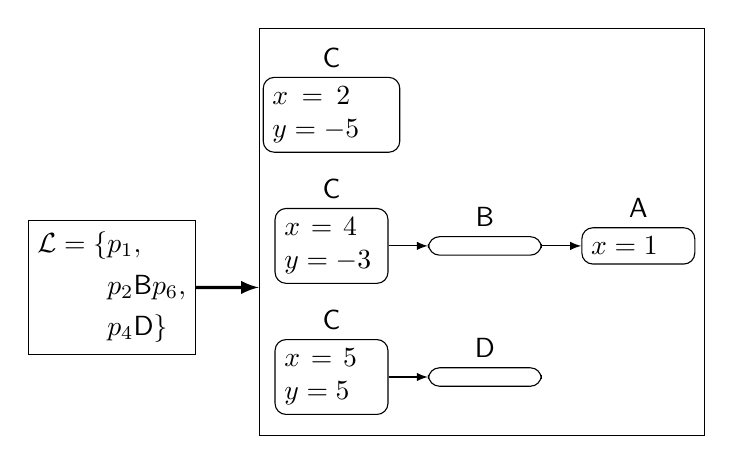
\begin{tikzpicture}[every initial by arrow/.style={text={},->>,thick},-latex,initial text={},node distance=2cm]


%%%%%%%%%%%%%%%%%%%%%% PRECEDENCE


\node[rectangle,draw] (L) {{$\begin{aligned}
\mathcal{L}=\{&p_1,\\
              &p_2\textsf{B}p_6,\\
			&p_4\textsf{D}\}
\end{aligned}$}};

\node (T1E1) [text width=1.5cm,above right=1.2cm of L]  [rectangle,draw,rounded corners,label=above:{\textsf{C}}] {$x=2$ $y=-5$};
    
\node (T2E1) [text width=1.2cm,below=.7cm of T1E1]  [rectangle,draw,rounded corners,label=above:{\textsf{C}}] {$x=4$ $y=-3$};
\node (T2E2) [text width=1.2cm,right=.5cm of T2E1]  [rectangle,draw,rounded corners,label=above:{\textsf{B}}] { };
\node (T2E3) [text width=1.2cm,right=.5cm of T2E2]  [rectangle,draw,rounded corners,label=above:{\textsf{A}}] {$x=1$ };

\node (T3E1) [text width=1.2cm,below=.7cm of T2E1]  [rectangle,draw,rounded corners,label=above:{\textsf{C}}] {$x=5$ $y=5$};
\node (T3E2) [text width=1.2cm,right=.5cm of T3E1]  [rectangle,draw,rounded corners,label=above:{\textsf{D}}] { };
 
\draw[-latex] (T2E1) -- (T2E2);
\draw[-latex] (T2E2) -- (T2E3);
\draw[-latex] (T3E1) -- (T3E2);
\coordinate (P47) at ($(T1E1.north)+(-.8,.5)$) ;
\coordinate (P48) at ($(T3E2.south)+(-.8,-.5)$) ;

\node[rectangle,draw,fit=(P47)(T2E3)(P48)] (Gen) {};
\draw[very thick,-latex] (L) -- (Gen.194);

\end{tikzpicture}
\end{document}